\subsection{Otras representaciones del problema}
Durante el desarrollo de este trabajo se han probado diferentes representaciones
del problema con el objetivo de buscar la que mejor se adapte al caso particular del FJSP. En
esta sección se van a explicar las diferentes representaciones que se han probado
y se han terminado por descartar, junto con una breve explicación de las razones
por las que se han descartado y que características de ellas se han aprovechado
para la representación final. Por último, se explicará de forma breve como se
modeló su espacio de estados y de acciones, y como se actualizaba el estado
de forma breve para cada una de ellas. 

\subsubsection{Representación con construcción secuencial}
Esta representación es la primera que se probó, y consiste en representar el
problema de una forma secuencial, es decir, cada operación se asigna a una máquina
en función de la información que se tiene en ese momento. Esta idea 
sentó las bases de como se podría representar el proceso de construcción de una
solución, pero se descartó por ser demasiado simple y tener problemas de escalabilidad,
ya que no existía una forma de proveer adecuadamente toda la información necesaria
para la toma de decisiones. A continuación, se explicara su implicación.

\begin{itemize}
    \item \textbf{Espacio de estados:} el estado es representado por una 
    lista de máquinas, donde cada máquina tiene una lista de operaciones asignadas
    a ella. Se utiliza una estructura de datos matricial donde se proporcionan estadísticas 
    sobre la maquina que esta asignada para representar este estado. Ademas, cada elemento de la lista 
    contiene información sobre las operaciones, su duración, prioridad u otras características relevantes.
    \item \textbf{Espacio de acciones:} Las acciones posibles consisten en asignar una operación 
    a una máquina específica o realizar un cambio de máquina. Es posible representar las acciones 
    mediante un conjunto de códigos que identifiquen cada operación. En este caso, las acciones
    disponibles se mostrarían junto a un código extra que representaría el cambio de máquina, este código
    tomo al valor de la ultima operación más uno.
    \item \textbf{Transiciones de estado:} Cuando el agente asigna una operación a una máquina, 
    el estado se actualiza con la nueva asignación. Si el agente decide cambiar de máquina, 
    el estado se actualiza para reflejar la nueva máquina activa y las operaciones pertinentes.
\end{itemize}

\subsubsection{Representación mediante imagen con eliminación}
Esta representación consiste en representar el problema mediante una imagen, donde
cada píxel representa el tiempo de finalización de una operación en una posición
específica. El modelo en cuestión se basa en ir eliminando las operaciones de la
imagen que se encuentran ya asignadas en las diferentes máquinas en todas las
posiciones, el objetivo es eliminar todas las operaciones sobrantes de la 
imagen.\medskip

Esta representación se descartó por ser demasiado compleja, ya que aunque
en un principio parecía que podría ser una buena representación debido a la naturaleza
gráfica del problema, la complejidad de la representación y la gran dimensionalidad de
la misma la hacían inviable. No se rescató ninguna característica de esta para la 
representación final, ya que no se encontró ninguna que pudiera ser útil. Aquí se
explicará de forma breve como se modeló.

\begin{itemize}
    \item \textbf{Espacio de estados:} El estado se representa por una imagen que contiene 
    los posibles tiempos de finalización de las operaciones. Existe una matriz de píxeles 
    para representar la imagen, donde cada píxel representa el tiempo asociado a una operación 
    en una posición específica. Por ejemplo, el valor de un píxel podría representar el tiempo 
    de finalización estimado de una operación en una determinada ubicación.
    \item \textbf{Espacio de acciones:} Las acciones posibles consisten en eliminar zonas de 
    la imagen. Puedes representar las acciones mediante coordenadas que delimitan un área a 
    eliminar en la imagen. Por ejemplo, una acción podría estar representada por las 
    coordenadas de dos esquinas de un rectángulo que define la zona a eliminar.
    \item \textbf{Transiciones de estado:} En este caso, cuando el agente elimina una zona de 
    la imagen, el estado se actualiza reflejando la nueva configuración de tiempos de finalización. 
\end{itemize}
\begin{figure}[ht]
    \centering
    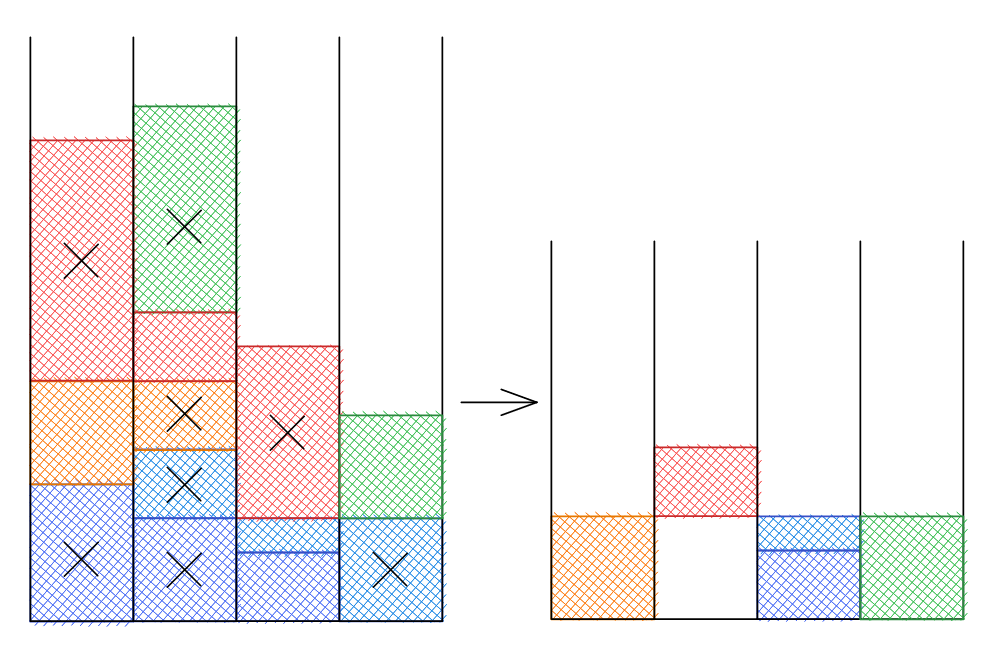
\includegraphics[scale=0.4]{image-rep.png}
    \caption{Representación mediante imagen con eliminación}
    \label{fig:image-rep}
\end{figure}

\subsubsection{Representación con grafos y nodo de cambio de máquina}
Por último, se decidió utilizar una representación basada en grafos, donde cada nodo
representa una operación y las aristas representan las dependencias entre ellas. Esta
representación se basa en la primera representación donde contábamos íbamos asignando
operaciones a máquinas, pero en este caso sustituimos esa representación matricial por
una representación mediante grafos. Esta representación no solo soluciona el problema
de la dimensionalidad de la representación, sino que además permite representar de
forma más sencilla las dependencias entre operaciones. Además, se mantiene la idea del
cambio de máquina con un nodo especial que representa el cambio y esta representación
es la que se ha utilizado en las versiones primerizas del modelo final.

\begin{itemize}
    \item \textbf{Espacio de estados:} cada estado se representa por un grafo 
    que representa la configuración actual de una máquina. Cada nodo del grafo puede representar 
    una operación, y las aristas representar las dependencias entre ellas. Se le asignan
    características a los nodos, como el tiempo de procesamiento de la operación o cualquier 
    otra información relevante.
    \item \textbf{Espacio de acciones:} las acciones posibles pueden ser cambiar de máquina 
    o realizar una operación en la máquina actual. Puedes representar las acciones mediante 
    un código que identifique cada operación y la maquina en la que se va a asignar. Por 
    ejemplo, una acción puede estar representada por un código que indique cambiar de máquina o 
    un código que indique realizar una operación específica en la máquina actual.
    \item \textbf{Transición de estado:} la transición de estado ocurren cuando el agente 
    toma una acción y el entorno se actualiza en consecuencia. Cuando se realiza una operación 
    en la máquina actual, el grafo de la máquina se actualiza para reflejar el cambio de estado. 
    Si se decide cambiar de máquina, se utiliza un nodo especial en el grafo para representar 
    la transición a otra máquina.
\end{itemize}
\begin{figure}[ht]
    \centering
    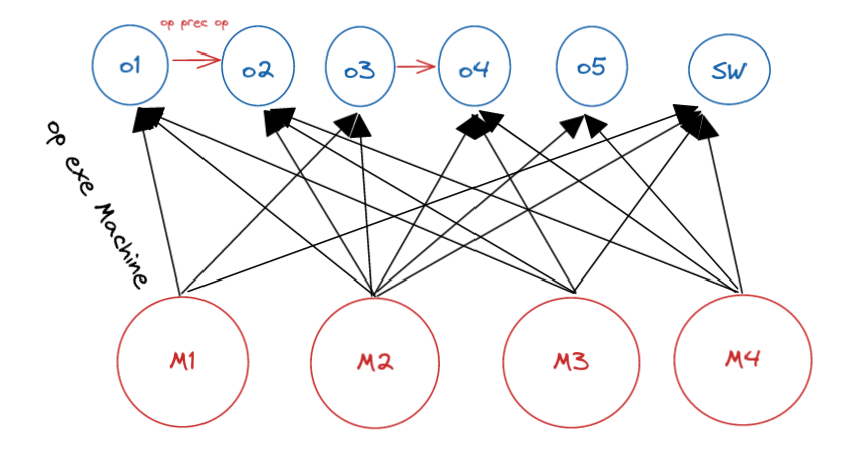
\includegraphics[scale=0.4]{graphv0.png}
    \caption{Representación mediante grafos con nodo de cambio de máquina}
    \label{fig:rep-graph-v0}
\end{figure}
